
\section{Introduction}

This note is a summary of work done for the Long Haul Network to USDF teats done on \jira{PREOPS-3571}.
This work was carried out in October 2023 - there may be more tests later.

\section {Test Setup}

To simulate as closely as possible the camera setup up eight of the camera nodes on the summit
were used to transmit data.

\subsection{Data}
Each node had some full focal plane image data on the local disk.
The chosen images were the pinhole images taken in 2020 since they have high information content and compress less than say flats from TS8.
The following  were provided by Tony Johnson :\\
\begin{tabular}{l l}
Romanesco  & MC\_C\_20200822\_000075\\
Vera\_Rubin & MC\_C\_20200822\_000054\\
Flammarion & MC\_C\_20200822\_000082\\
Group\_Photo & MC\_C\_20200822\_000061\\
\end{tabular}

The images are compressed but not in the way we are doing them now (gzip vs. Rice tile).  Same file would go from 25MB to 20MB, so this test is extra-conservative.

These images may also be found in {\tt LSSTCam}  butler repo on USDF  using:
\begin{verbatim}
  repo = 'LSSTCam'
  instrument = 'LSSTCam'
  collections=[f"{instrument}/raw/all"]
  butler = Butler(repo, collections=collections, instrument=instrument)

  where="exposure.obs_id IN ('MC_C_20200822_000075', 'MC_C_20200822_000054',
                             'MC_C_20200822_000082', 'MC_C_20200822_000061')}"

  datasetRefs = list(butler.registry.queryDatasets(datasetType='raw',where=where))

\end{verbatim}

There are 820 raw's in the collection.

\subsection{Sending  and Scripts} \label{sec:setup}

All scripts may be found in \url{https://github.com/lsst-dm/s3daemon}

A pooled connection S3 writer called {\tt s3daemon} was provided for K.T. Lim.
This was run on the background on each node.

The test client  {\tt send.py} can send one file and store it in S3 at the USDF with the given key.

The test scripts are in the summittests folder of the s3daemon repo.
Check this out where you want to run the scripts - all run from inside the summittests folder.
All scripts rely on a set of environment variables set in {\tt envvars.sh} this is not checked in but {\tt envvars\_template.sh} gives the variables minus the actual S3 keys. Copy this and get the keys from s3df.

On the summit for any of these to work you need to execute {\tt kinint} to allow ssh between nodes.
This must be done on each login.

The scripts need to be on all the nodes {\tt pushToNodes.sh} distributes them.\\
{\tt runOnNodes.sh ./runS3Daemon.sh} is used to run the daemon on all nodes simultaneously.\\
{\tt runOnNodes.sh ./sendTest.sh} is used to run that on all nodes simultaneously.

These  are all the support scripts:
\begin{itemize}
\item {\tt gatherLogs.sh} pulls back the log files from each node to logs folder on main node
\item {\tt pushToNodes.sh} pushes the s3daemon folder to all nodes.
\item {\tt runs3Daemon.sh} runs the daemon and sets up a log file using the hostname.
\item {\tt runOnNodes.sh ./runs3daemon.sh} is used to run that on all 8 nodes .
\item {\tt readFile.sh}  read  single file from disk
\item {\tt readTest.sh}  run a loop like sendTest to show reading is not a bottleneck
\item {\tt report.py}  read log file(s) summaries and plot histogram of times
\item {\tt sendTest.sh} uses {\tt send.py} to send 20 files simultaneously from the Test folder set up by Tony.
\item {\tt stops3daemon.sh}  use pkill to kill the daemon
\end{itemize}


\section{October 2023 test} \label{sec:oct2023}
Using the setup as described in \secref{sec:setup} from {\tt lsstcam-dc01} in  {\tt ~womullan}
the s3daemon was run on : {\tt
 lsstcam-dc03 lsstcam-dc04 lsstcam-dc05 lsstcam-dc06 lsstcam-dc07 lsstcam-dc08 lsstcam-dc09 lsstcam-dc10
}

The sendTest was then executed on each node with 20 repeats:
\begin{verbatim}
./runOnNodes.sh ./sendTest.sh 20
\end{verbatim}
There are only 64 files on node 10 not 108 as on the other nodes.
Since the script simply repeats sending all files a number of times this resulted in significantly less files from node 10.
In the next iteration this will be made total number of sends rather than repeat all.
Hence {\tt ./sendTest 14} was
additionally run on that node to get he same number of files sent and a few lines removed from the log.
This was run after the end of the test so the times are better on that node which should be taken a a single node test..

The log files were all pulled back to {\tt lsstcam-dc1} :
\begin{verbatim}
./gatherLogs.sh
\end{verbatim}
The results are below in \secref{sec:summit}

To check the read time on the local disk  and eliminate this as a potential bottleneck:
\begin{verbatim}
./readTest.sh 1
Just read total 20
Reading /home/tonyj/Test/MC_C_20200822_000054/MC_C_20200822_000054_R00_SW1.fits 1 seconds
Reading /home/tonyj/Test/MC_C_20200822_000054/MC_C_20200822_000054_R00_SW0.fits 1 seconds
Reading /home/tonyj/Test/MC_C_20200822_000054/MC_C_20200822_000054_R01_S00.fits 2 seconds
Reading /home/tonyj/Test/MC_C_20200822_000054/MC_C_20200822_000054_R00_SG1.fits 2 seconds
Reading /home/tonyj/Test/MC_C_20200822_000054/MC_C_20200822_000054_R00_SG0.fits 2 seconds
Reading /home/tonyj/Test/MC_C_20200822_000054/MC_C_20200822_000054_R00_SG0.fits 2 seconds
Reading /home/tonyj/Test/MC_C_20200822_000054/MC_C_20200822_000054_R01_S10.fits 2 seconds
Reading /home/tonyj/Test/MC_C_20200822_000054/MC_C_20200822_000054_R01_S02.fits 2 seconds
Reading /home/tonyj/Test/MC_C_20200822_000054/MC_C_20200822_000054_R02_S00.fits 2 seconds
Reading /home/tonyj/Test/MC_C_20200822_000054/MC_C_20200822_000054_R02_S02.fits 2 seconds
Reading /home/tonyj/Test/MC_C_20200822_000054/MC_C_20200822_000054_R02_S01.fits 2 seconds
Reading /home/tonyj/Test/MC_C_20200822_000054/MC_C_20200822_000054_R01_S01.fits 2 seconds
Reading /home/tonyj/Test/MC_C_20200822_000054/MC_C_20200822_000054_R01_S11.fits 2 seconds
Reading /home/tonyj/Test/MC_C_20200822_000054/MC_C_20200822_000054_R01_S21.fits 2 seconds
Reading /home/tonyj/Test/MC_C_20200822_000054/MC_C_20200822_000054_R02_S12.fits 2 seconds
Reading /home/tonyj/Test/MC_C_20200822_000054/MC_C_20200822_000054_R02_S20.fits 2 seconds
Reading /home/tonyj/Test/MC_C_20200822_000054/MC_C_20200822_000054_R01_S22.fits 2 seconds
Reading /home/tonyj/Test/MC_C_20200822_000054/MC_C_20200822_000054_R01_S12.fits 2 seconds
Reading /home/tonyj/Test/MC_C_20200822_000054/MC_C_20200822_000054_R02_S10.fits 2 seconds
Reading /home/tonyj/Test/MC_C_20200822_000054/MC_C_20200822_000054_R01_S20.fits 2 seconds
Reading /home/tonyj/Test/MC_C_20200822_000054/MC_C_20200822_000054_R02_S11.fits 2 seconds

\end{verbatim}


To check the s3 writing on the s3df was not a problem a single node test  was run on sdfrome002 using
a set of the images retrieved from the s3 and written to {\tt /tmp/Test}. {\tt envvars.sh} was set up approately and the following commands run:
\begin{verbatim}
make venv
./runs3daemon
./sendTest

INFO 2023-10-18 08:32:44,341 __main__ - 1697643163.739425 0.601705 sec
INFO 2023-10-18 08:33:04,043 __main__ - 1697643183.774607 0.269175 sec
INFO 2023-10-18 08:36:03,866 __main__ - 1697643363.024261 0.842190 sec
INFO 2023-10-18 08:36:03,936 __main__ - 1697643363.000797 0.935841 sec
INFO 2023-10-18 08:36:04,138 __main__ - 1697643363.139490 0.998814 sec
INFO 2023-10-18 08:36:04,153 __main__ - 1697643362.611110 1.542599 sec
INFO 2023-10-18 08:36:04,157 __main__ - 1697643362.859598 1.298039 sec
INFO 2023-10-18 08:36:04,170 __main__ - 1697643363.229397 0.940939 sec
INFO 2023-10-18 08:36:04,181 __main__ - 1697643363.092925 1.088640 sec
INFO 2023-10-18 08:36:04,275 __main__ - 1697643362.768593 1.507033 sec
INFO 2023-10-18 08:36:04,289 __main__ - 1697643362.587150 1.702505 sec
INFO 2023-10-18 08:36:04,316 __main__ - 1697643362.676797 1.639230 sec
INFO 2023-10-18 08:36:04,327 __main__ - 1697643362.634262 1.693653 sec
INFO 2023-10-18 08:36:04,419 __main__ - 1697643362.543653 1.875807 sec
INFO 2023-10-18 08:36:04,484 __main__ - 1697643363.277188 1.207678 sec
INFO 2023-10-18 08:36:04,485 __main__ - 1697643362.812599 1.672884 sec
INFO 2023-10-18 08:36:04,558 __main__ - 1697643362.957474 1.600601 sec
INFO 2023-10-18 08:36:04,579 __main__ - 1697643362.906880 1.672704 sec
INFO 2023-10-18 08:36:04,594 __main__ - 1697643363.047643 1.547244 sec
INFO 2023-10-18 08:36:04,772 __main__ - 1697643362.724061 2.048239 sec
INFO 2023-10-18 08:36:04,784 __main__ - 1697643362.498078 2.286714 sec
INFO 2023-10-18 08:36:05,023 __main__ - 1697643363.184669 1.838420 sec
INFO 2023-10-18 08:36:23,957 __main__ - 1697643383.051293 0.906635 sec
INFO 2023-10-18 08:36:23,998 __main__ - 1697643383.140353 0.857726 sec
INFO 2023-10-18 08:36:24,052 __main__ - 1697643383.074861 0.977346 sec
INFO 2023-10-18 08:36:24,200 __main__ - 1697643383.323820 0.876308 sec
INFO 2023-10-18 08:36:24,211 __main__ - 1697643383.232854 0.979019 sec
INFO 2023-10-18 08:36:24,212 __main__ - 1697643383.007916 1.204627 sec
INFO 2023-10-18 08:36:24,226 __main__ - 1697643383.276831 0.949985 sec
INFO 2023-10-18 08:36:24,273 __main__ - 1697643383.188520 1.085285 sec
INFO 2023-10-18 08:36:24,399 __main__ - 1697643382.962684 1.436435 sec
INFO 2023-10-18 08:36:24,502 __main__ - 1697643383.097912 1.404957 sec
\end{verbatim}

The log file was pulled to the local machine and the plot is in \secref{sec:s3df}

\section{Results}
\subsection{SLAC } \label{sec:s3df}

The summary for the slac test is plot in \figref{fig:slac} :
\begin{verbatim}
sdfrome002 32 files Mean:1.30 max:2.29 min: 0.27 std:0.44, var:0.19 seconds
\end{verbatim}

\begin{figure}
\begin{centering}
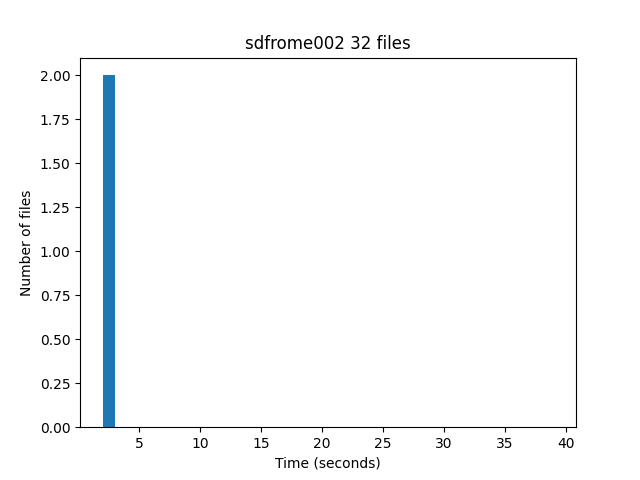
\includegraphics[width=0.8\textwidth]{plots/sdfrome002}
	\caption{Writing 20 files in 20 threads to the s3 on SLAC shows no appreciable slow down.
\label{fig:slac}}
\end{centering}
\end{figure}

\subsection{Summit } \label{sec:summit}

The summary for the summit logs are here with plots below:
\begin{verbatim}
lsstcam-dc03 2268 files Mean:14.79 max:42.44 min: 4.53 std:6.93, var:48.04 seconds
lsstcam-dc04 2268 files Mean:16.68 max:48.73 min: 3.97 std:7.47, var:55.82 seconds
lsstcam-dc05 2268 files Mean:17.65 max:48.35 min: 3.75 std:7.30, var:53.28 seconds
lsstcam-dc06 2268 files Mean:17.46 max:43.75 min: 3.98 std:7.65, var:58.54 seconds
lsstcam-dc07 2268 files Mean:16.77 max:45.88 min: 4.34 std:7.23, var:52.20 seconds
lsstcam-dc08 2268 files Mean:16.15 max:46.57 min: 4.58 std:6.98, var:48.74 seconds
lsstcam-dc09 2268 files Mean:13.46 max:42.95 min: 4.43 std:6.87, var:47.13 seconds
lsstcam-dc10 2268 files Mean:6.88 max:22.08 min: 3.61 std:3.19, var:10.20 seconds
all 18144 files Mean:14.98 max:48.73 min: 3.61 std:7.60, var:57.83 seconds
\end{verbatim}


\begin{figure}
\begin{centering}
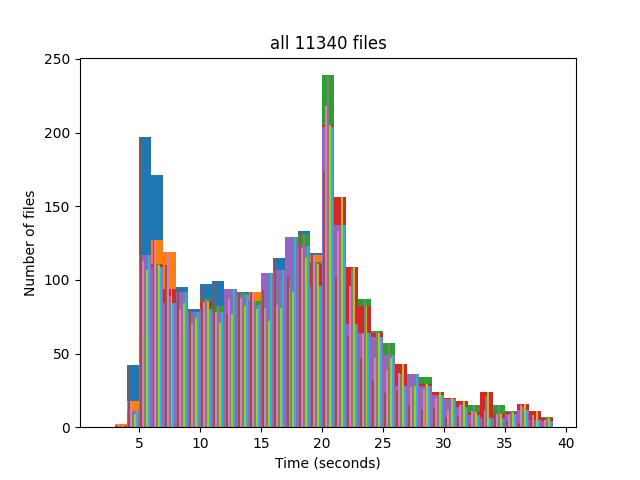
\includegraphics[width=0.8\textwidth]{plots/all}
	\caption{Combined plot of send times from all nodes.
\label{fig:summit}}
\end{centering}
\end{figure}


\begin{figure}
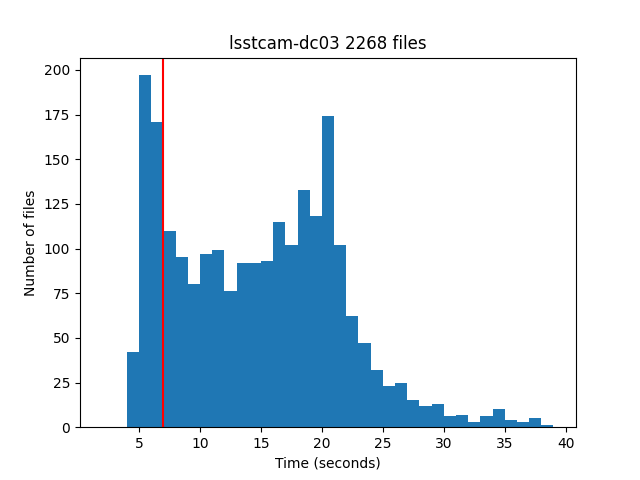
\includegraphics[width=0.4\textwidth]{plots/lsstcam-dc03}
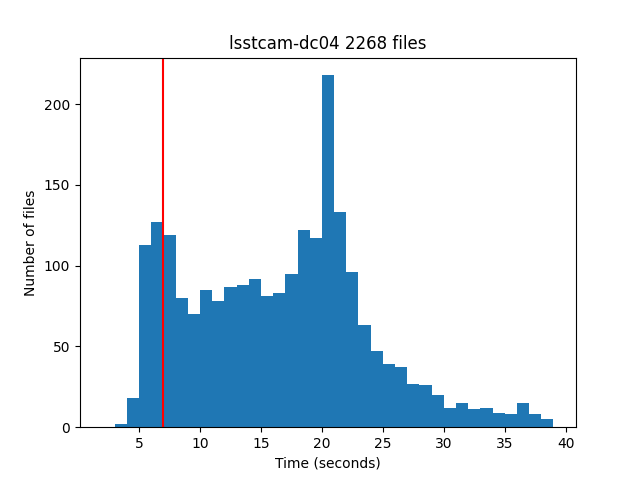
\includegraphics[width=0.4\textwidth]{plots/lsstcam-dc04}\\
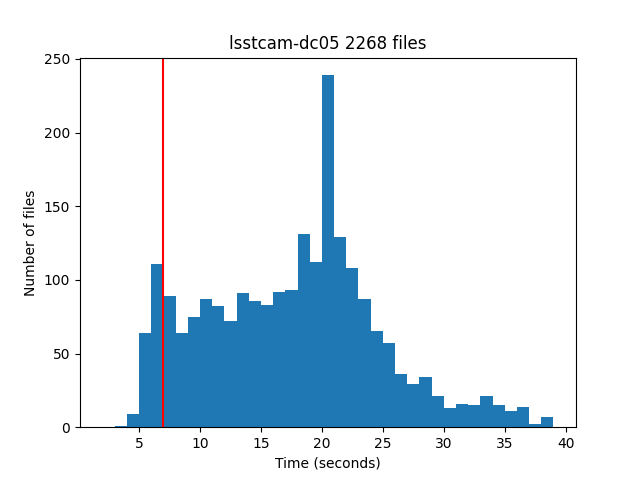
\includegraphics[width=0.4\textwidth]{plots/lsstcam-dc05}
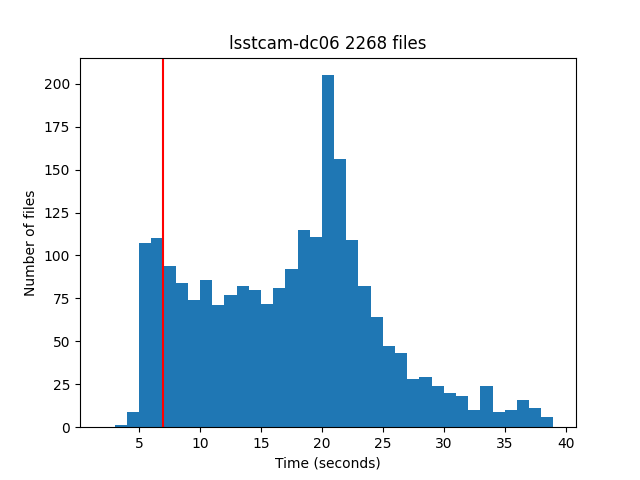
\includegraphics[width=0.4\textwidth]{plots/lsstcam-dc06}
\end{figure}

\begin{figure}
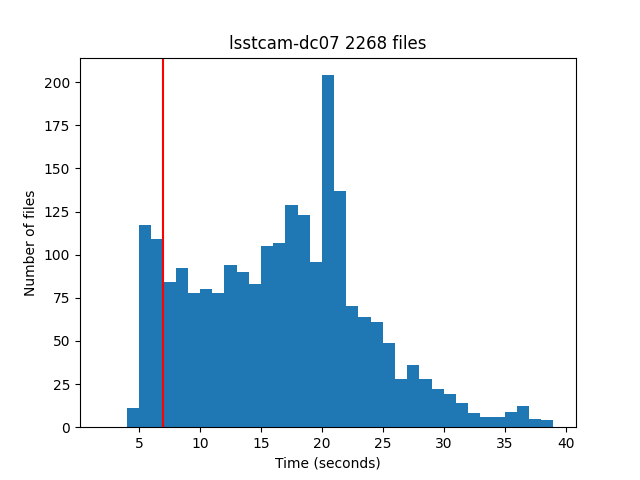
\includegraphics[width=0.4\textwidth]{plots/lsstcam-dc07}
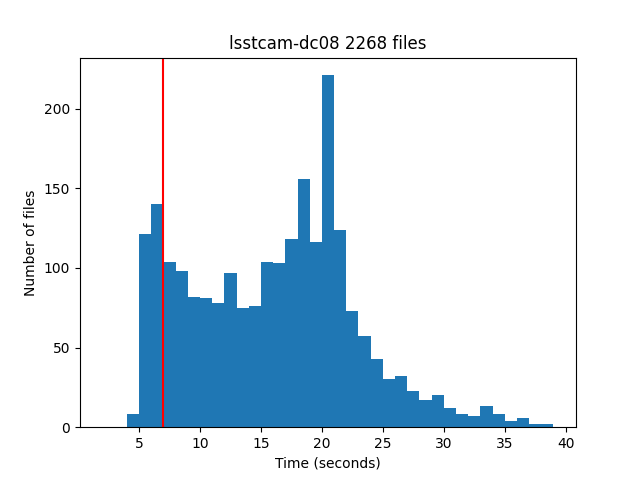
\includegraphics[width=0.4\textwidth]{plots/lsstcam-dc08}\\
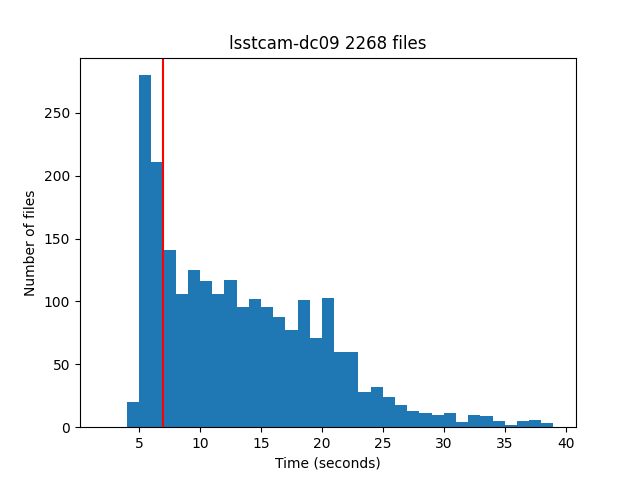
\includegraphics[width=0.4\textwidth]{plots/lsstcam-dc09}
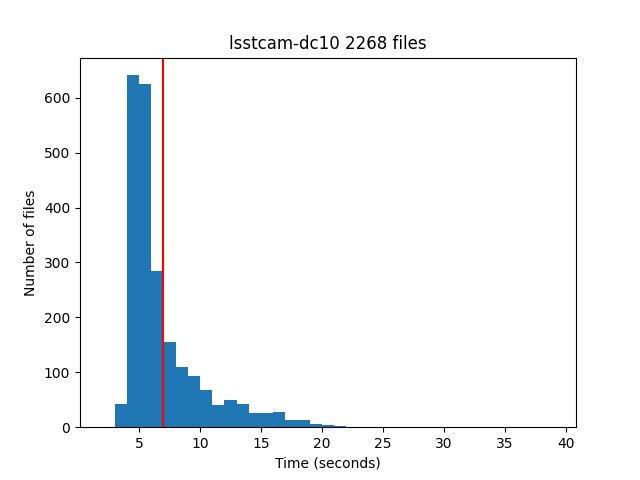
\includegraphics[width=0.4\textwidth]{plots/lsstcam-dc10}
\end{figure}

\section{Conclusion}
Looking at the results of the October test we can see some files do indeed arrive in USDF in 4 or 5 seconds.
Hence it is possible to send many files at high speed to the USA.
Specifically looking at node 10 which was run independently we see more than half the 2K files arrive in under 7 seconds.
However we need all files to arrive in under 7 seconds and as we run on multiple nodes we see the times stretch out to 48 seconds.
Even with node 10 as a single test we see some  files taking 20s.
Two other tests, the read test (\secref{sec:oct2023})  and write test (\secref{sec:s3df}),  show this is not a problem on the origin nor destination nodes.
Hence we are left with the path in between - routers, firewalls and the LHN.
Further tests are needed to find the bottleneck.
